\subsection{DIAGRAMM}
\begin{figure}[H]
  \centering
  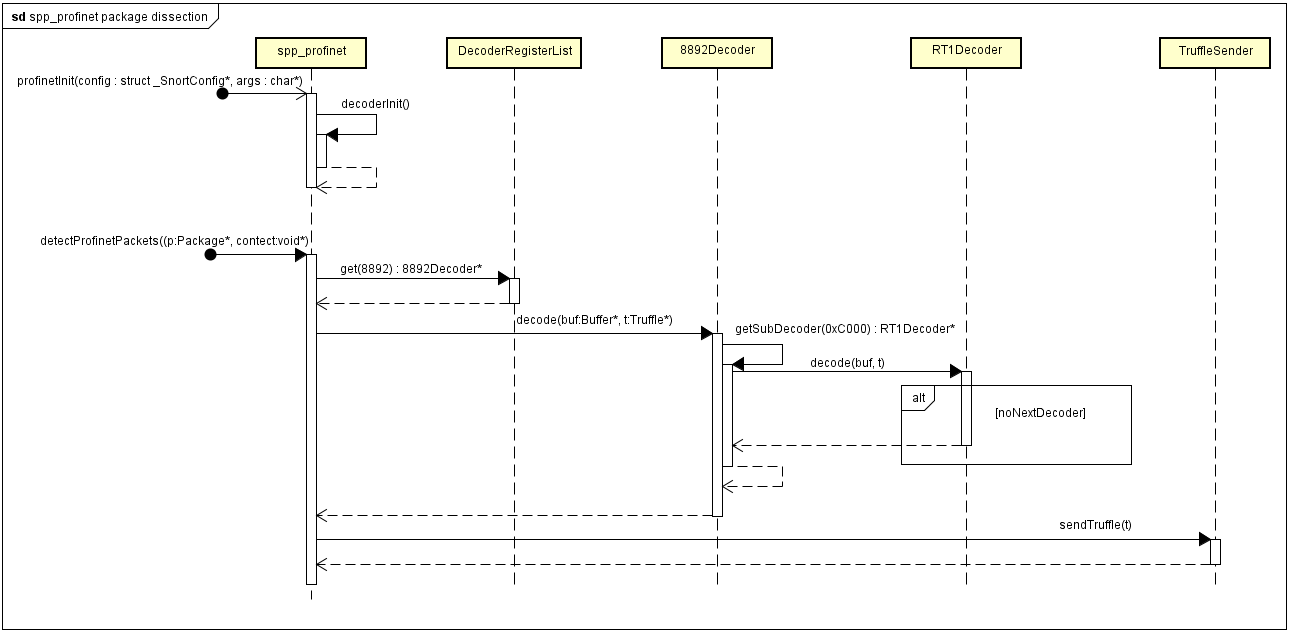
\includegraphics[width=\textwidth]{../diagramimages/spp-profinet-package-dissection.png}
  \caption[Sequenzdiagramm DIAGRAMM]{Sequenzdiagramm DIAGRAMM}
\end{figure}

Hier geht es um die Speicherroutine der Commands und Snapshots des Graphen. Beim Start des ReplayLogSaveService erstellt sich dieser einen Replay-, Command- und Snapshotlogger um sich später einen ReplayLog zusammenzustellen. Der ReplayLogSaveService ist ein Listener beim TruffleReceiver, wodurch die eingehenden Commands im CommandLogger gespeichert werden können. Jeweils nach einem bestimmten Zeitintervall in der Endlosschleife wird ein Snapshot von dem Graphen erstellt und zusammen mit den gesammelten Commands in einem ReplayLog serialisiert. 